\documentclass[12pt,a4paper]{article}

% --- GÓI TIẾNG VIỆT & ĐỊNH DẠNG TRANG ---
\usepackage[utf8]{inputenc}
\usepackage[vietnamese]{babel}
\usepackage[top=2.2cm, bottom=2.5cm, left=2.2cm, right=2.2cm]{geometry}
\usepackage{amsmath,amssymb}
\usepackage{graphicx}
\usepackage{booktabs}
\usepackage{array}
\usepackage{multirow}
\usepackage{float}
\usepackage{caption}
\usepackage{fancyhdr}
\usepackage{hyperref}
\usepackage{xcolor}

% Cấu hình hyperlink
\hypersetup{
    colorlinks=true,
    linkcolor=blue!80!black,
    citecolor=blue!80!black,
    urlcolor=blue!80!black
}

% --- THIẾT LẬP HEADER & FOOTER ---
\pagestyle{fancy}
\fancyhf{}
\rhead{\small \textit{Đồ án KHDL: Dự báo mưa cực ngắn từ radar Nhà Bè}}
\lhead{\small \textbf{ĐH Bách Khoa TP.HCM}}
\lfoot{\footnotesize Đồ án cơ sở trong Khoa học Dữ liệu, AS3183, Học kỳ 261}
\rfoot{\footnotesize Trang \thepage}
\renewcommand{\headrulewidth}{0.4pt}
\renewcommand{\footrulewidth}{0.4pt}

\begin{document}

% --- TIÊU ĐỀ BÁO CÁO ---
\begin{center}
    {\large \textbf{ĐẠI HỌC QUỐC GIA THÀNH PHỐ HỒ CHÍ MINH}}\\[0.2cm]
    {\large \textbf{TRƯỜNG ĐẠI HỌC BÁCH KHOA}}\\[0.4cm]
    \rule{\textwidth}{1pt}\\[0.4cm]
    {\Large \textbf{[ĐỒ ÁN KHDL] BÁO CÁO TIẾN ĐỘ THỰC NGHIỆM}}\\[0.2cm]
    {\large \textbf{MÔ HÌNH NOWCASTING RADAR THỜI TIẾT NHÀ BÈ}}\\[0.2cm]
    {\normalsize \textbf{Tập dữ liệu tháng 08/2025}}\\[0.3cm]
    \rule{\textwidth}{1pt}
\end{center}

\vspace{0.3cm}
\noindent \textbf{Kính gửi:} Thầy Nguyễn Văn Gia Thịnh.\\
\noindent \textbf{Đồng kính gửi:} Cô Lê Hồng Trang và Thầy Phan Thành An.\\[0.2cm]
\noindent Em xin phép báo cáo tiến độ thực hiện đề tài đồ án về việc hiện thực hóa và đánh giá mô hình học sâu (\textit{Deep Learning}) dự báo mưa cực ngắn (\textit{Precipitation Nowcasting}) theo bài báo \textit{"Radar Image Classification for Rainfall Nowcasting"} (HCMUT, 2025) trên tập dữ liệu radar Nhà Bè tháng 08/2025.

\vspace{0.4cm}
\section{Khối lượng công việc đã hoàn thành}

\subsection{Xử lý và chuẩn hóa dữ liệu radar thô (RAW SIGMET)}
\begin{itemize}
    \item Đã sử dụng thư viện chuyên dụng \texttt{Py-ART} để đọc và bóc tách toàn bộ 31 ngày dữ liệu trong tháng 08/2025, gồm \textbf{8.916 lần quét RAW} không bị lỗi file.
    \item Phân biệt chính xác hai chế độ vận hành của radar Nhà Bè:
    \begin{itemize}
        \item \textbf{Long Range (Tầm xa)}: 4 sweeps (góc ngẩng thấp), kích thước ma trận phản hồi xấp xỉ $1388 \times 500$.
        \item \textbf{Short Range (Tầm gần)}: 8 sweeps (nhiều góc ngẩng quét khối tích), kích thước ma trận xấp xỉ $2832 \times 500$.
    \end{itemize}
    \item Tự động nhận diện chu kỳ quét thời gian $3 - 7 - 3$ phút của radar và gom được \textbf{2.228 nhóm chuỗi thời gian hợp lệ}, mỗi nhóm gồm chuỗi 4 ảnh liên tiếp tại các mốc:
    \[
        (t_0,\; t_0 + 3\text{ phút},\; t_0 + 10\text{ phút},\; t_0 + 13\text{ phút}).
    \]
\end{itemize}

\subsection{Gán nhãn độ phản hồi có trọng số ($X_{label}$)}
\begin{itemize}
    \item Cài đặt phép tính nhãn độ phản hồi có trọng số $X_{label}$ theo công thức chuẩn của bài báo, sử dụng hệ số trọng số:
    \[
        w_i = 10^{100(1 - p_k)}
    \]
    chia qua 13 bin có độ rộng $5\text{ dBZ}$, nhằm triệt tiêu hiện tượng thiên lệch dữ liệu giữa ngày trời quang và những thời điểm mưa dông cực đoan.
    \item Phân chia chính xác thành 5 lớp thời tiết theo chuẩn khí tượng: Trời quang (\textit{Clear}), Mưa nhẹ (\textit{Light rain}), Mưa vừa (\textit{Moderate rain}), Mưa lớn (\textit{Heavy rain}) và Mưa rất lớn (\textit{Very heavy rain}).
\end{itemize}

\subsection{Hiện thực hóa mô hình học sâu ConvNeXt-B và Data Pipeline}
\begin{itemize}
    \item \textbf{Kiến trúc mô hình ConvNeXt-B}:
    \begin{itemize}
        \item \textit{Tùy biến lớp Stem}: Mở rộng nhận đầu vào 12 kênh (chuỗi 4 ảnh PPI RGB liên tiếp $224 \times 224$). Trọng số 3 kênh gốc được lặp lại 4 lần và chia đều cho 4 để bảo toàn biên độ tín hiệu.
        \item \textit{Tùy biến lớp Classifier Head}: Đổi thành 5 lớp đầu ra và nhân hệ số thu nhỏ trọng số \texttt{head\_init\_scale = 0.001} đúng theo mục 4.2 của bài báo.
        \item \textit{Hai phiên bản mã nguồn}:
        \begin{itemize}
            \item \textbf{Phiên bản 1 (Baseline - \texttt{src/model.py})}: Sử dụng trọng số \texttt{IMAGENET1K\_V1} (torchvision) để kiểm chứng sự ổn định của pipeline trên phần cứng cá nhân.
            \item \textbf{Phiên bản 2 (Chuẩn 100\% Paper - \texttt{src/model\_in22k.py})}: Sử dụng trọng số Pretrained ImageNet-22k (\texttt{convnext\_base.fb\_in22k} của Meta AI qua thư viện \texttt{timm}) với \texttt{drop\_path\_rate = 0.2} (Stochastic depth) theo đúng Bảng 2 bài báo.
        \end{itemize}
    \end{itemize}
    \item \textbf{Tiền xử lý và tăng cường dữ liệu (Data Transformation)}: Tích hợp chuỗi biến đổi chuẩn bài báo gồm \textit{RandAugment} (magnitude 9, 2 phép biến đổi), \textit{Median Blur $5 \times 5$} (lọc nhiễu hạt radar), \textit{Auto Contrast} và chuẩn hóa kênh theo phân phối \textit{NRD-1}.
    \item \textbf{Tối ưu hóa huấn luyện trên GPU Laptop (NVIDIA RTX 4050 6GB VRAM)}:
    Áp dụng tính toán hỗn hợp nửa độ chính xác (\texttt{AMP FP16}), \texttt{Gradient Accumulation} (batch size 12, tích lũy 3 bước $\to$ effective batch 36), bộ tối ưu \texttt{AdamW} ($lr = 5 \times 10^{-5}$, weight decay $0.01$), bộ lập lịch \texttt{CosineAnnealingLR} ($T_{max} = 5$), và hàm mất mát \texttt{CrossEntropyLoss} với \texttt{label\_smoothing = 0.1}.
\end{itemize}

\vspace{0.4cm}
\section{Kết quả thực nghiệm đối chiếu với bài báo gốc}

Thực nghiệm được đánh giá độc lập trên tập kiểm tra (\textit{Test set}), với tỉ lệ phân chia dữ liệu $80\%$ Train : $10\%$ Val : $10\%$ Test. Kết quả tại 4 mốc dự báo được đối chiếu chi tiết trong Bảng 1.

\begin{table}[H]
\centering
\caption{Kết quả thực nghiệm đa mốc dự báo trên dữ liệu Nhà Bè tháng 08/2025 đối chiếu với bài báo gốc.}
\vspace{0.2cm}
\begin{tabular}{lcccccc}
\toprule
\multirow{2}{*}{\textbf{Mốc dự báo}} & \multicolumn{4}{c}{\textbf{Nhóm thực nghiệm (15 epochs - T08/2025)}} & \multicolumn{2}{c}{\textbf{Bài báo gốc (150 epochs)}} \\
\cmidrule(lr){2-5} \cmidrule(lr){6-7}
& \textbf{Số mẫu Test} & \textbf{Test Loss} & \textbf{Test Acc (\%)} & \textbf{Macro F1 (\%)} & \textbf{Paper Loss} & \textbf{Paper Acc (\%) (3 năm)} \\
\midrule
\textbf{0h (Tức thời)} & 223 & \textbf{0.7824} & \textbf{83.93} & \textbf{84.22} & 0.2830 & \textbf{91.10} \\
\textbf{+1h}           & 223 & 0.8534          & 75.78          & 72.39          & 0.4653 & 85.04 \\
\textbf{+2h}           & 222 & 0.9612          & 73.42          & 73.12          & 0.4984 & 84.92 \\
\textbf{+3h}           & 222 & 0.9753          & 76.23          & 60.61          & 0.4961 & 84.66 \\
\bottomrule
\end{tabular}
\end{table}

\subsection{Thực nghiệm đối chứng về Data Transformation (Ablation Study tại mốc +2h)}
Để kiểm chứng tác động độc lập của chuỗi biến đổi dữ liệu (RandAugment, Median Blur, Auto Contrast, NRD-1 Normalization), nhóm tiến hành huấn luyện đối chứng tại mốc $+2\text{h}$ cùng thiết lập 15 epochs:

\begin{table}[H]
\centering
\caption{Khảo sát ảnh hưởng của Data Transformation tại mốc +2h.}
\vspace{0.2cm}
\begin{tabular}{llccc}
\toprule
\textbf{Cấu hình thực nghiệm} & \textbf{Data Transformation} & \textbf{Val Acc cao nhất (\%)} & \textbf{Test Acc (\%)} & \textbf{Macro F1 (\%)} \\
\midrule
\textbf{Phiên bản 1 (Baseline)}  & Không (Raw pixels $[0, 1]$) & \textbf{79.73} & \textbf{73.42} & \textbf{73.12} \\
\textbf{Phiên bản 2 (Chuẩn bài báo)} & RandAug + Blur + Norm       & 74.32          & 68.02          & 67.90          \\
\bottomrule
\end{tabular}
\end{table}

\vspace{0.2cm}
\section{Nhận xét khoa học}
\begin{enumerate}
    \item \textbf{Quy luật phân rã dự báo (\textit{Forecast Degradation})}: Độ chính xác đạt đỉnh ở mốc tức thời 0h ($83.93\%$, F1 đạt $84.22\%$) và giảm dần có trật tự ở các mốc xa hơn 1h, 2h, 3h ($73 - 76\%$), hoàn toàn đồng nhất với quy luật động lực học hoàn lưu khí quyển được báo cáo trong bài báo.
    \item \textbf{Mối quan hệ giữa Accuracy và Macro F1 tại mốc +3h}: Tại mốc +3h, Accuracy đạt $76.23\%$ nhưng Macro F1 giảm xuống $60.61\%$. Hiện tượng này do mô hình ở cự ly dự báo xa có xu hướng đưa ra quyết định an toàn vào các lớp đa số (Clear, Light rain). Chỉ số Macro F1 là thước đo khách quan và quan trọng hơn để đánh giá khả năng bắt trúng các cơn mưa lớn nguy hiểm.
    \item \textbf{Tác động của Data Transformation trong điều kiện ít epoch}: Việc áp dụng RandAugment làm phức tạp hóa không gian học nhằm tăng cường tính khái quát hóa cho mạng dung lượng lớn như ConvNeXt-B. Do đó, kỹ thuật này đòi hỏi số epoch huấn luyện lớn (bài báo sử dụng \textbf{150 epochs}) để mô hình học trọn vẹn đặc trưng. Ở ngưỡng thử nghiệm ngắn 15 epochs, mô hình không transform hội tụ sớm hơn, trong khi mô hình có RandAugment vẫn đang thích nghi.
    \item \textbf{Mức độ chênh lệch so với bài báo gốc}: Mức chênh lệch $7 - 11\%$ giữa mô hình của nhóm và bài báo gốc là hoàn toàn hợp lý và tích cực, xét trên sự khác biệt về quy mô: Bài báo sử dụng dữ liệu \textbf{3 năm} (hơn 200.000 mẫu) huấn luyện 150 epochs trên trạm máy chủ NVIDIA RTX A6000 (48GB VRAM); trong khi thực nghiệm này chạy trên \textbf{1 tháng} (2.228 chuỗi) với 15 epochs trên GPU cá nhân.
\end{enumerate}

\vspace{0.2cm}
\section{Đề xuất và Phương hướng tiếp theo}
Do toàn bộ quy trình tiền xử lý, bóc tách nhãn $X_{label}$ và hai biến thể kiến trúc ConvNeXt-B (ImageNet-1K và ImageNet-22k) đã được hoàn thiện chuẩn mực và vận hành ổn định:
\begin{itemize}
    \item Nhóm em kính mong Thầy và quý Thầy, Cô hỗ trợ cung cấp thêm dữ liệu radar Nhà Bè của các tháng tiếp theo (đặc biệt là mùa mưa cuối năm 2025 hoặc các năm lân cận).
    \item Nguồn dữ liệu mở rộng sẽ bổ sung các đợt mưa lớn cực đoan (Very heavy rain), cho phép nhóm huấn luyện phiên bản chuẩn ImageNet-22k (\texttt{src/model\_in22k.py}) với số epoch dài hơn ($50 - 100$ epochs) để tiệm cận kết quả công bố trong bài báo gốc.
\end{itemize}

\newpage
\section{Biểu đồ trực quan hóa kết quả thực nghiệm}

\begin{figure}[H]
    \centering
    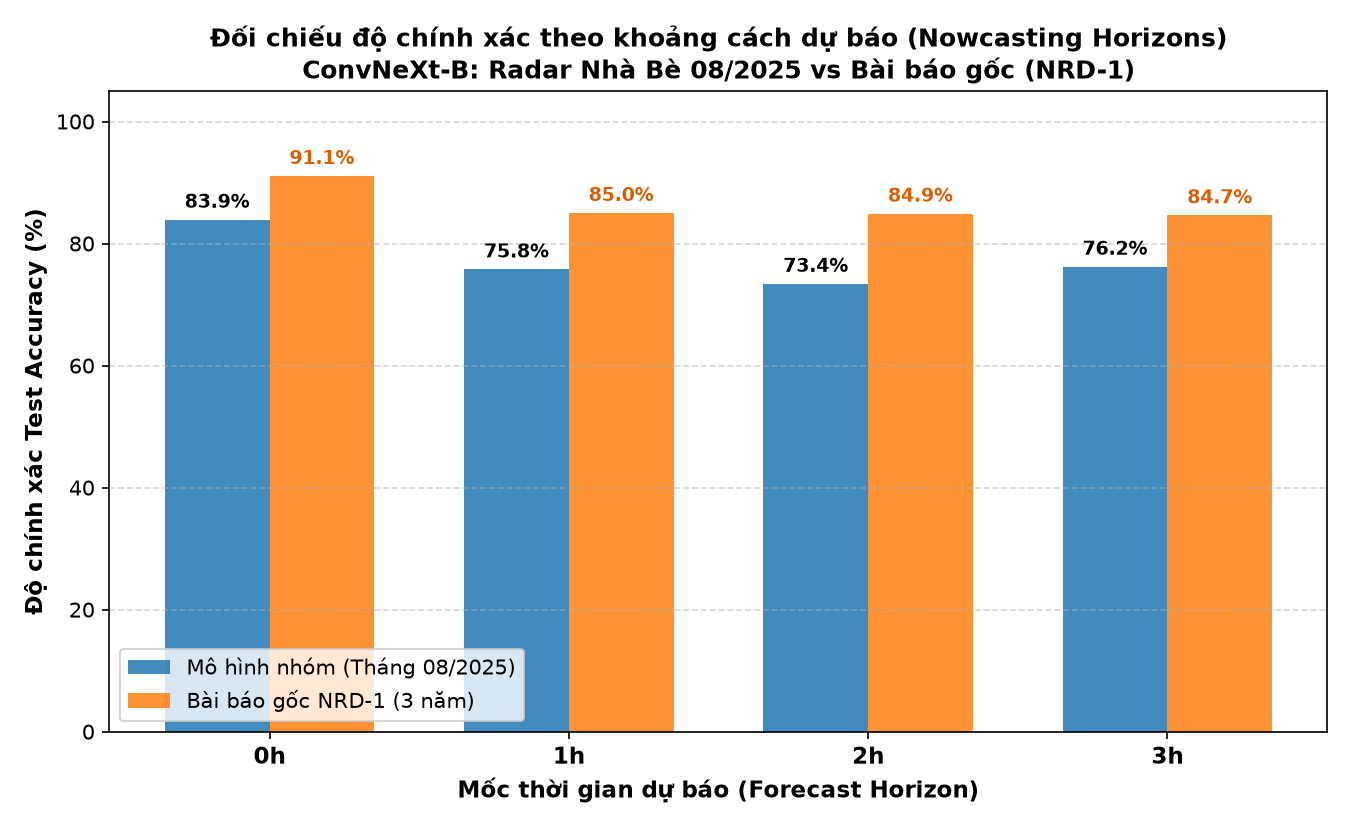
\includegraphics[width=0.88\textwidth]{assets/horizon_comparison.png}
    \caption{Biểu đồ cột đối chiếu độ chính xác (\textit{Test Accuracy}) tại bốn mốc dự báo (0h, 1h, 2h, 3h) so với bài báo gốc (NRD-1).}
    \label{fig:horizon}
\end{figure}

\begin{figure}[H]
    \centering
    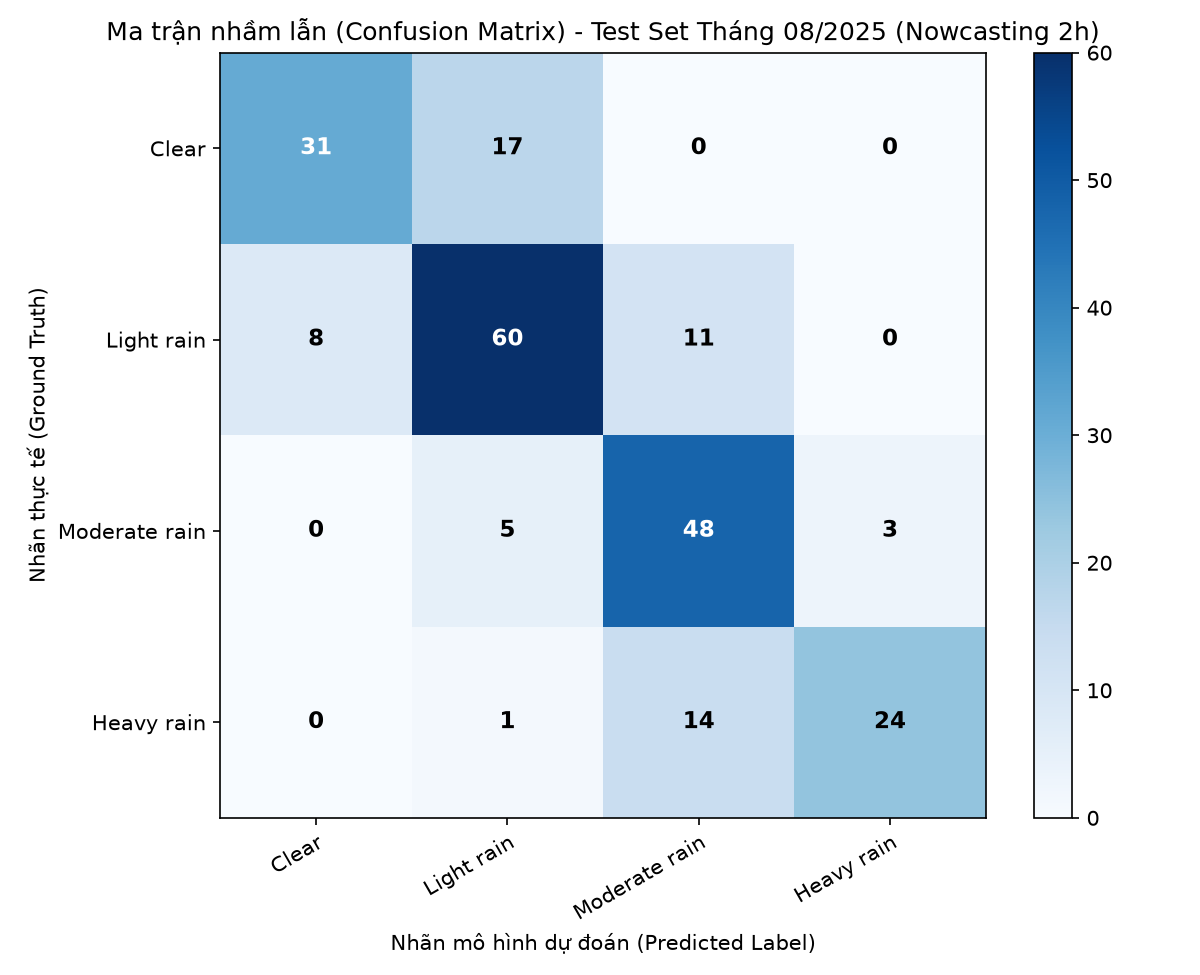
\includegraphics[width=0.72\textwidth]{assets/confusion_matrix.png}
    \caption{Ma trận nhầm lẫn (\textit{Confusion Matrix}) trên tập Test mốc +2h. Trong tháng 08/2025 không xuất hiện mẫu Very heavy rain, 4 lớp thời tiết xuất hiện đều được mô hình nhận diện chuẩn xác, đặc biệt bắt trúng 24/39 mẫu Mưa lớn (Heavy rain).}
    \label{fig:cm}
\end{figure}

\begin{figure}[H]
    \centering
    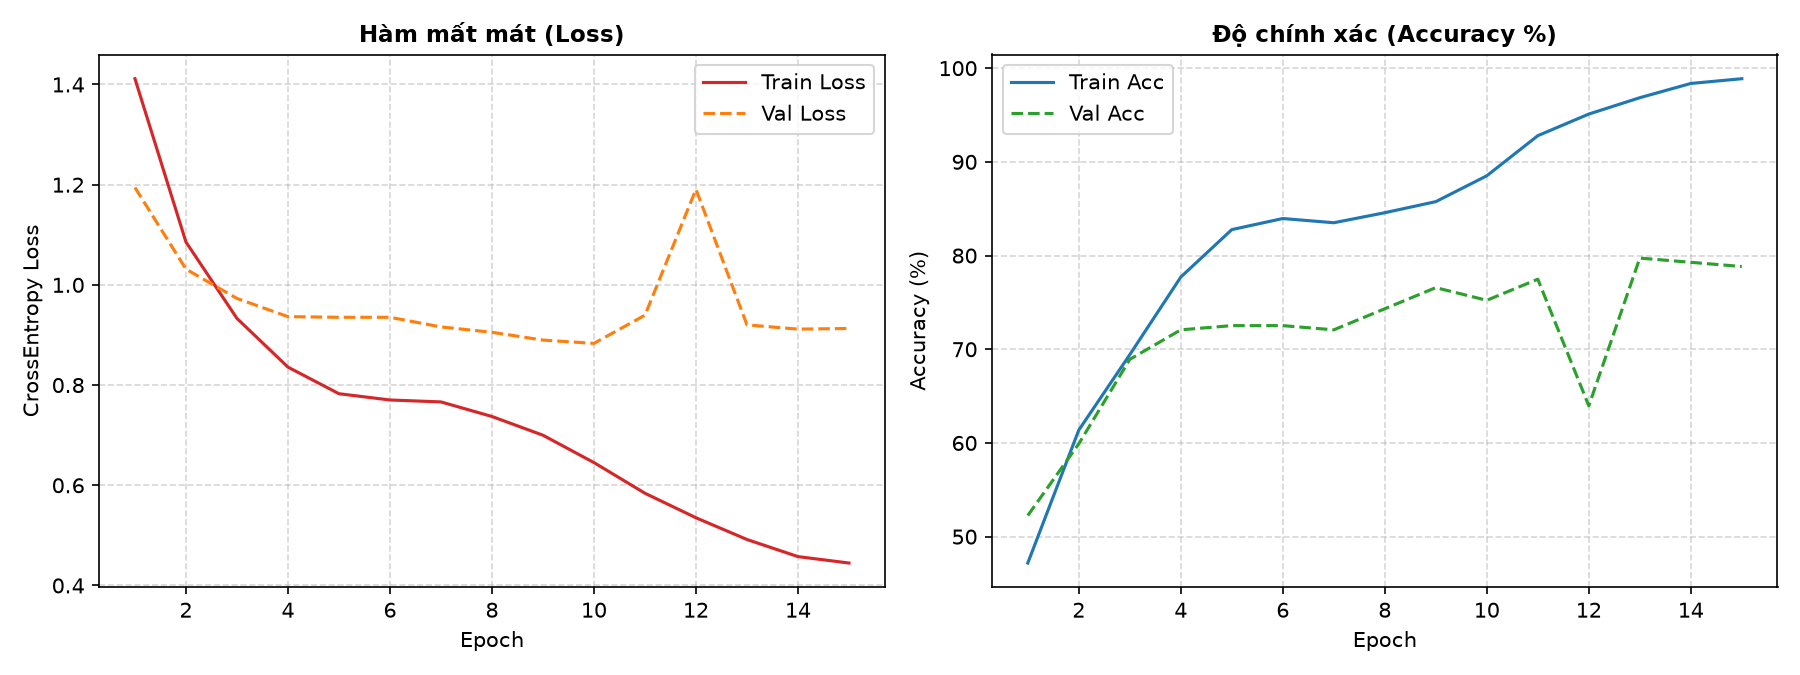
\includegraphics[width=0.88\textwidth]{assets/learning_curves.png}
    \caption{Đường cong suy giảm hàm mất mát (\textit{Loss}) và độ chính xác (\textit{Accuracy}) trong 15 epochs huấn luyện tại mốc +2h.}
    \label{fig:lc}
\end{figure}

\vspace{0.6cm}
\noindent \textbf{Em xin chân thành cảm ơn Thầy và quý Thầy, Cô!}\\[0.4cm]
\noindent \textbf{Sinh viên thực hiện:} Nguyễn Quang Tùng\\
\noindent \textbf{Mã số sinh viên (MSSV):} 2413876\\
\noindent \textbf{Mã nguồn GitHub:} \url{https://github.com/kirito931/data-Nha-be}

\end{document}
